
%
%  $Description: Author guidelines and sample document in LaTeX 2.09$ 
%
%  $Author: ienne $
%  $Date: 1995/09/15 15:20:59 $
%  $Revision: 1.4 $
%

\documentclass[times,10pt,twocolumn]{article} 
\usepackage{epsfig}
\usepackage{latex8}
\usepackage{listings}
\usepackage{subfigure}
\usepackage{times}
\usepackage{url}

%\documentstyle[times,art10,twocolumn,latex8]{article}

%------------------------------------------------------------------------- 
% take the % away on next line to produce the final camera-ready version 
\pagestyle{empty}

%------------------------------------------------------------------------- 
\begin{document}

\title{User-level Grid Monitoring with Inca 2}

\author{Shava Smallen, Kate Ericson, Jim Hayes, Catherine Olschanowsky \\
San Diego Supercomputer Center\\ University of California, San Diego\\ 
9500 Gilman Drive, La Jolla, CA 92093-0505, USA\\ 
\{ssmallen,kericson,jhayes,cmills\}@sdsc.edu\\
}

\maketitle
\thispagestyle{empty}

%1.  Motivate and differentiate the Grid monitoring Inca does
%2. Describe Inca 2 design and its benefits
%3. Illustrate that Inca 2 design is mature and being used in production by
%several Grids
%4. Be different from Inca 1 paper

\begin{abstract}
User-level Grid monitoring is valuable, how it relates to other Grid
monitoring,  and what are its implementation challenges.
Inca 1 good but had limitations.  In this paper, we introduce Inca 2 and
describe its features and architecture.  We then show a few use cases for Inca
is being deployed on TeraGrid and XXX?  System impact results and performance
results.  Finally, we discuss our future work.  
\end{abstract}

%------------------------------------------------------------------------- 
\Section{Introduction}

% Standard "Grids are good" intro paragraph.  But are complex.  
Grid systems provide unified and coherent access to distributed computing,
data storage and analysis, instruments, and other resources.  These systems
require the careful coordination of software packages, services, and
configurations across multiple, heterogeneous resources.  The TeraGrid
project~\cite{teragrid}, for example, manages the coordination of software and
services by deploying and monitoring a common user environment across
distributed, heterogeneous resources. The organization of TeraGrid software
and services is referred to as the Common TeraGrid Software and Services
(CTSS).  TeraGrid's software and services uniformity simplifies access to its
resources, which consist of more than 102 teraflops of compute capability and
more than 15 petabytes of online storage, all interconnected by a network that
can transfer a terabyte of data in under 10 minutes.  

% Complex means they are difficult to provide and maintain. Describe the
% stakeholders.   Monitoring is needed.
Providing and maintaining a stable infrastructure for these complex 
Grid systems poses challenges for both administrators who build and
maintain Grid resources and scientists who use them.  First, system
administration is distributed across multiple administrative domains 
requiring a significant amount of coordination.  This is typically performed by
a group of Grid operators who take into account local site policies 
and decide when software (including updates and patches) should be deployed to
resources and how it should be configured for the set of heterogeneous
resources.  Each site's system administrators, who are oftentimes not Grid
experts, are then responsible for providing the required Grid software
components and services for their resource and debugging any problems that
arise.  Well-defined requirements and good communication are required in this
model.  Otherwise inconsistencies between the resources arise that either
inconvenience the user or prevent them from using particular resources
together.  Second, as a large distributed system, failures will occur over
time in the Grid services due to network or system failures, software
misconfiguration, or software bugs.  In order to detect such problems, 
monitoring of the resources is required.  

% What types of Grid monitoring are around and what the limitations are
One approach to monitoring Grids, used by tools such as
MonALISA~\cite{monalisa} and GridICE~\cite{gridice}, is to aggregate and
display data from existing cluster or system administrator monitoring tools
such as Ganglia~\cite{ganglia}, CluMon~\cite{clumon}, and
Nagios~\cite{nagios}.  This provides a centralized, systems-level view of Grid
resources where low-level host statistics and queue information can be
examined.  This type of monitoring information is useful for showing the
utilization of Grid resources, however, it does not provide the type of
high-level monitoring needed to detect user problems within the Grid
infrastructure, such as incompatible software versions.  

% What user-level monitoring provides and why we think it is good
User-level Grid monitoring approaches testing and performance measurement of
the Grid infrastructure from the user perspective.  The goal is to act as an
impartial test user of the Grid and detect problems with the infrastructure so
they can be fixed before users notice them -- user complaints should not be
the first indication of Grid failures.  We refer to an executable program that
tests or measures some aspect of a system or installed software from the
user-perspective as a reporter.  In our view, the following guidelines 
define user-level Grid monitoring: 

\begin{itemize}

\item In order to reflect regular user experiences, tests or performance
measurements of the Grid infrastructure should be done from a standard user
account.  In fact, it is important to not execute under a system
administrator's account because they may be privileged and often have custom
shell initialization files.

\item Also in order to reflect regular user experiences, tests should be
written and configured using information directly from user documentation
(e.g., hostnames, ports, pathnames, etc.).  This may not always be possible
when documentation and testing are done in parallel in a pre-production
environment but they should be closely coordinated activities. 

\item Since Grids are dynamic, user-level tests or performance measurements
should be automated and executed periodically.

\item Tests or performance measurements that interact with Grid services
require authentication and should be executed using a standard user GSI
credential that is mapped to the standard user account.  

\item Tests or performance measurements should be executed locally on all Grid
resources when appropriate so that all Grid access points available to users
are verified.  Similarly, it is important to execute some tests all-to-all
in order to detect site-to-site configuration errors such as authentication
problems.

\end{itemize}

\noindent In our experience, writing and maintaining user-level tests and
performance measurements is an iterative refinement process since Grids are
dynamic and the software environment changes over time as packages are
upgraded.  It is also difficult to write and deploy a test perfectly the first
time because of portability issues and sometimes incomplete user
documentation.  For example, it may take a few iterations to determine whether
detected failures are the result of a faulty test, fault user documentation,
or a faulty system.  Realistically, this is a labor-intensive activity and
thus the amount of user-level Grid monitoring is often limited by the amount
of people resources that can be assigned to it.  However, A good goal is to
test all the commands that exist in the user documentation and/or have at
least one basic test for each software component of the Grid infrastructure.  

% Inca 1~\cite{inca1} first addressed user-level Grid monitoring but had
% limitations.  We learned lessons from our TeraGrid deployment and
% developed Inca 2.
In 2003, SDSC, in partnership with TeraGrid, began developing Inca
1~\cite{inca1} to implement a user-level monitoring system with the above
features and started using it to validate and
verify that CTSS was deployed consistently across all TeraGrid resources and
to monitor its status.  At that time, the only available user-level Grid
monitoring tools were the NCSA TestGrid script~\cite{ncsa-test} and
GITS~\cite{gits}, scripts that run a fixed number of Grid tests and output
results in HTML.  Although these tools were easy to install and produced
useful information, they showed only the view of the Grid from a single
resource, lacked automation, and were not easily extensible.  The initial
version of Inca was implemented as a client-server architecture.  It provided
data collection, data storage (with limited archiving capabilities) that was
accessible from a Web services interface, and data display though Web status
pages.  Inca was first deployed to TeraGrid in mid 2003 and released in late
2003. After running Inca 1 for a year and a half on TeraGrid, we learned some
valuable lessons and designed Inca 2, our current release.  Inca 2
contains a number of substantial improvements over Inca 1 with respect to
security, installation and maintenance, and storage capabilities.  A
production release of Inca 2 was provided in February 2007 and has been
running on TeraGrid since November 2006.  Currently, seven other Grids in the
U.S., Europe, and Australia use Inca.  

% This motivated our development of a new version of Inca.
In the next section, we describe the features of Inca 2 and note which
are new features based on our experiences with deploying Inca 1 on TeraGrid.
We then describe the Inca 2 architecture and how it can be used to provide
user-level Grid monitoring.  In Section~\ref{usecases}, we describe two 
uses of Inca 2 for Grid software environment verification and benchmarking.  
Finally, we describe some future work and summarize the paper.

%------------------------------------------------------------------------- 
\Section{Inca 2 Features}
  
% Philosophy of user-level testing
% Practical byproducts
The main goal of the Inca 2 design was to XXX (general, flexible, easy to
install, deploy, and
maintain, scalable, secure).
The following lists the key features of Inca 2 noting which are new features
to Inca 1 versus improved.

\begin{enumerate}

\item Collects a wide variety of user-level monitoring results (e.g., simple
test data to more complex performance benchmark output).  (improved) 

\item Captures the context of a test or benchmark as it executes (e.g.,
executable name, inputs, source host, etc.) so that system administrators have
enough information to understand the result and can troubleshoot system
problems without having to know the internals of Inca 2. (improved)

\item Provides facilities to ease the process of writing test or benchmarks,
deploying them into Inca 2 installations, and sharing them with other Inca 2
users.  

\item Periodic tests executed by the monitoring system should be automated and
run from a standard user account.  A user GSI credential should be issued and
used by the monitoring system to test services that require authentication.  
%myproxy stuff
\item Tests should be executed locally on all Grid resources when appropriate so
that all Grid access points available to users are tested.  
\item The configuration of tests should be managed centrally in order to ensure
consistent testing of the resources, rather than by system administrators who
may not use the same information that is available to users.
\item The testing system should easily adapt to new resources and testing
requirements.  In our experience, testing has an iterative refinement process
because Grids are dynamic and the software environment changes over time as
packages are upgraded.  Furthermore, it is often difficult to write and deploy
a test perfectly the first time because of portability issues and incomplete
user documentation.   
\item System administrators should not need to know the details of the
monitoring system in order to troubleshoot problems.  When a problem is
detected the monitoring system should provide system administrators with
sufficient information to locate the problem easily and test repairs.
\item A history of test results (especially any error messages) should be
retained in order to understand the behavior of their Grid over time. This
history should be available through a flexible querying interface.
\item A running monitoring system should have a limited impact on the resources
it measures and should be secure.
\end{enumerate}

%------------------------------------------------------------------------- 
\Section{Inca 2 Architecture}

\begin{figure*}[htb]
  \centering
  \mbox{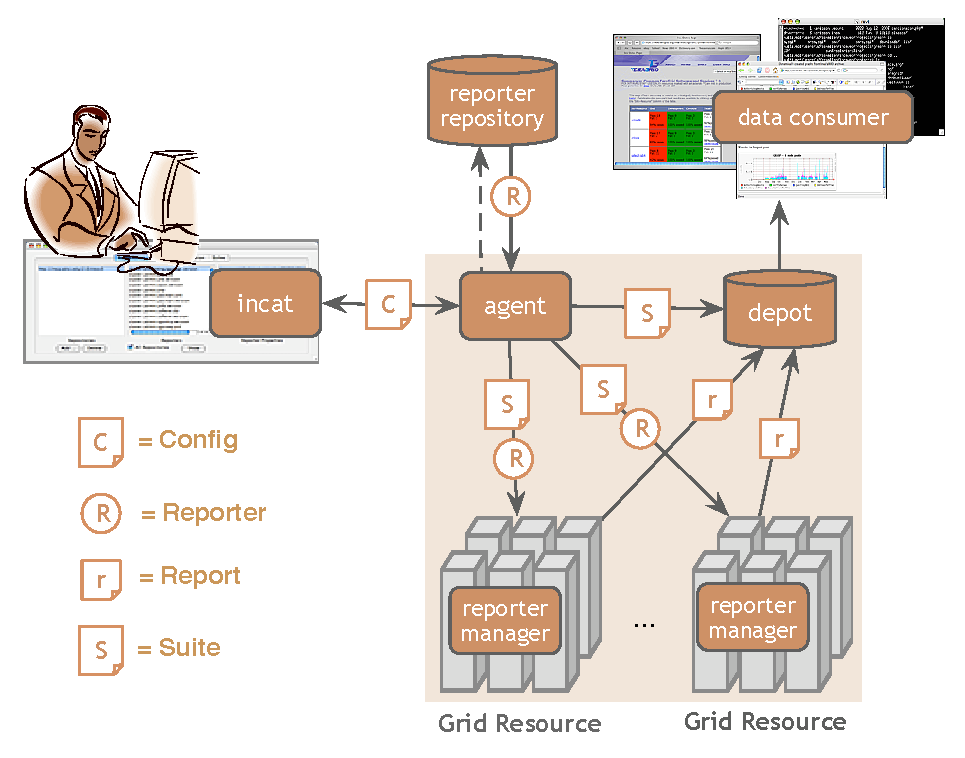
\epsfig{file=arch.eps, width=.8\textwidth}}
  \caption{\label{arch_fig} Inca architecture.}
\end{figure*}

% overview description of components
Figure~\ref{arch_fig} shows the architecture of Inca 2 designed to implement
the features described in the previous section.  Inca 2 is composed of 3 core
components (in highlighted box):  the agent, depot, and reporter manager.
The \textit{agent} and \textit{reporter managers} coordinate the execution of
tests and performance measurements on the Grid resources and the
\textit{depot} stores and archives the results.  The inputs to Inca 2 are one
or more \textit{reporter repositories} that contain user-level tests and
benchmarks called \textit{reporters} and a configuration file describing how
to execute them on the Grid resources created using an administration GUI tool
called \textit{incat} (Inca Administration Tool).  The output or results
collected from the resources are queried by the \textit{data consumer} and
displayed to users.  The following steps describe how an Inca administrator
would deploy user-level test and/or performance measurements to their
resources.

\begin{enumerate}

\item Using the guidelines described in the introduction, the Inca
administrator either writes reporters to monitor their Grid or uses existing
reporters in a published repository.

\item The Inca administrator creates a deployment configuration file that
describes the user-level monitoring for their Grid using incat and submits it
to the agent.

\item The agent
  \begin{enumerate}
    \item fetches reporters from the reporter repository
    \item creates a reporter manager on each resource
    \item sends the reporters and instruction for executed them to each reporter manager.
  \end{enumerate}

\item Each reporter manager executes reporters according to its schedule and
sends results (reports) to the depot

\item Data consumers display collected data (reports) by querying the depot
\end{enumerate}

\noindent The following subsections describe the Inca components in more
detail using the order of the steps above.

\SubSection{Reporters}

\lstset{
  basicstyle=\scriptsize\ttfamily, 
  frame=single,
  keywordstyle=\textbf, 
  identifierstyle=, 
  commentstyle=\scriptsize\ttfamily, 
  stringstyle=\ttfamily, 
  numbers=left, 
  numberstyle=\scriptsize,
  stepnumber=2,
  firstnumber=1,
  showstringspaces=false} 
\begin{figure}
\lstset{language=Perl} 
\subfigure[]{\lstinputlisting{grid.globus.gramPing}}
\lstset{language=XML,keywordstyle={}} 
\subfigure[]{\lstinputlisting{grid.globus.gramPing.out}}
\caption{\label{pingReporter}(a) An Inca reporter that tests the user-level
availability of a Globus GRAM server and (b) its sample output.}
\end{figure}

An Inca reporter is an executable program that tests or measures some aspect
of a system or installed software.   Reporter executables are designed to be
easy to produce and can be run outside of the Inca system (e.g., by a system
administrator).  A reporter should be written following the user-level
monitoring guidelines described in the introduction and could be a simple
Globus~\cite{globus} GRAM gatekeeper ping test (see Figure~\ref{pingReporter})
or a more complex Grid application benchmark~\cite{grasp}.  Reporters must
support certain command line options and produce an XML document or report
according to the Inca reporter schema.  The goal of the reporter schema is to
accommodate multiple types of data and to capture information about the
reporter execution to diagnose any detected failures.  The reporter schema
consists of the following elements: 

\begin{itemize}
\item a set of header tags describing the context of the reporter
execution:  GMT timestamp, hostname, reporter name, reporter version, working
directory, reporter path, and arguments;
\item an optional set of debug or information log tags similar to log4j~\cite{log4j} output;
\item a body containing the results expressed as any XML sequence; and
\item an exit status tag
indicating whether the reporter was able to complete its test or measurement
and an optional error message.  
\end{itemize} 
\noindent Because the body of the report can be any XML sequence, it enables
reporters to express a wide variety of information.  Today, we have four
standard body schemas to express software version information, software
functionality or service tests results, usage information, and performance
results.  

We provide an extensible set of Perl APIs to handle much of the effort of
writing reporters.  Figure~\ref{pingReporter} shows (a) an Inca reporter that
pings a pre-WS Globus GRAM server and (b) its corresponding output when
executed on a local machine.  The reporter uses two of the Perl APIs:
Inca::Reporter::SimpleUnit (which is a subclass of Inca::Reporter) and
Inca::Reporter::GridProxy.  The Inca::Reporter API provides convenience
functions for handling the required input arguments
(lines~\ref{pingReporter}(a) 12-14 $\rightarrow$ lines \ref{pingReporter}(b)
10-31) and printing the Inca-compliant header and exit status XML tags
(lines\ref{pingReporter}(a) 4-11, 24 $\rightarrow$ \ref{pingReporter}(b)
1-9,43-46).  It also includes some informational and debug logging functions
again similar to log4j; the log output has been very useful to system
administrators who can view a summary of the test or benchmark that the
reporter performed without reading the reporter source code.  Line
\ref{pingReporter}(a) 15 shows a special log function, loggedCommand, that
executes a system command (using a 30 second timeout) and logs to the 'system'
level of the log XML output (lines \ref{pingReporter}(b) 32-36).  The subclass
Inca::Reporter::SimpleUnit is the API responsible for printing the simplest
standard reporter body schema -- reporting software functionality or service
tests results; it handles the printing of the small body XML
(lines~\ref{pingReporter}(b) 39-41) using the functions unitSuccesss
(line~\ref{pingReporter}(a) 22) or unitFailure (lines~\ref{pingReporter}(a)
18, 20) depending on the output of system command.  Finally, the
Inca::Reporter::GridProxy API (line~\ref{pingReporter}(a) 3) adds a proxy
dependency to the reporter telling the Inca system to download a
short-term proxy before running this reporter (this is discussed further in
Section~\ref{proxy}).  Most current reporters use the Perl APIs and consist of
fewer than 30 lines of code.

\SubSection{Reporter Repositories}

The Inca agent retrieves reporters from collections called reporter
repositories that consist of reporters, required packages and libraries,
and a catalog file. Repository contents are accessible using a URL and can
be shared across multiple Inca deployments. The Inca team publishes a
reporter repository that contains reporters developed for TeraGrid.  

\SubSection{Inca administration GUI tool (incat)}

The Inca administrative GUI tool (incat) is the main interface by which an
Inca administrator interacts with the Inca system.  Incat allows the Inca
administrator to view the choose which resources to monitor and which tests or 
benchmarks to deploy to those resources.  The following subsections
describe the Inca components that are configurable via incat.  
To configure reporter execution, an Inca administrator launches a GUI tool,
called incat.  Incat allows the administrator to choose which resources to
monitor and which reporters to deploy to those resources.  For each
reporter, the administrator can specify the resources to run on,
command-line arguments, the runtime environment, the frequency of execution,
and resource limits. The Inca administrator may also group related reporters
into suites that can be shared across different Inca deployments.  This can
be useful to determine interoperability among Grids or to determine whether
an application's requirements are being fulfilled on a Grid.

\subsubsection{Suites}
%\subsubsection{Series}

\subsubsection{Resource Macros}

\SubSection{Agent}

The Inca agent is a server that implements the configuration specified by the
Inca administrator.  After determining which Inca tests should be executed on
each resource, the agent stores this configuration information in the depot.
It then stages and launches a dependent component, called a reporter manager,
on each resource using either SSH or Globus [13].  Once a reporter manager
contacts its agent, the agent transmits Inca tests to execute, along with
their dependencies, configuration and schedule of execution. 
  

\SubSection{Reporter Manager}

The Inca reporter manager is a lightweight process responsible for managing
the schedule and execution of Inca tests, called reporters, on a single
resource. The reporter manager receives reporter updates and dependencies
(e.g., Inca Perl APIs or source code) from the agent along with requests for
reporter scheduling changes.  Running under a regular user account, the
reporter manager executes reporters on-demand or using an internal cron
scheduler, and sends reports to the depot for archiving. The reporter
manager monitors reporter system usage and enforces limits (e.g., wall clock
time, CPU time, memory).  System usage information is sent to the depot with
each report. 



\SubSection{Depot}

The Inca depot server is responsible for storing configuration information
and the data produced by reporters. The depot maintains a relational
database via Hibernate [14] so that it can use a variety of databases.  The
depot provides full archiving of reporter output and structures its schema
to reduce redundant data.  Data can be queried using SQL queries. Predefined
queries exist to return the latest report instances of a suite, a single
report instance, or a report history.  A Web services interface is also
available to provide unauthenticated query access to data.  


\SubSection{Data Consumer}

The Inca data consumer is a Web application that queries the Inca depot for
data and displays it in a user-friendly format.  The data consumer is
packaged with Jetty [15] so that pages can be served immediately without
deploying Tomcat [16].  A set of JSP tags and pages query the Inca depot for
data (returned as XML) and a set of XSL stylesheets format the data as HTML.

~\newpage
~\newpage
~\newpage
~\newpage
%------------------------------------------------------------------------- 

\Section{Use Cases}
\label{usecases}

\SubSection{TeraGrid}

\subsubsection{Description and Requirements}

% Describe CTSS 

\subsubsection{Usage of Inca}

% Describe reporters, configuration, and deployment.  Figure.

\subsubsection{Results}

% Consumer view of CTSS, security, etc.

~\newpage

\SubSection{GrASP}

\subsubsection{Description and Requirements}

% Describe GrASP probes

\subsubsection{Usage of Inca}

% Used to deploy GrASP probes to Grids.  Probes wrapped as reporters (maybe
% right in future as though we already included GrASP as a dependency cause
% it should be done by June.

\subsubsection{Results}

% A paper.  Interesting that error messages were important.  Predictions?

~\newpage

\SubSection{Other uses}
~\newpage
%------------------------------------------------------------------------- 
\Section{Future Work}

\SubSection{Graphing and Summary Statistics}

\SubSection{Knowledge Base}

\SubSection{Fault Tolerance}
~\newpage

%------------------------------------------------------------------------- 
\Section{Summary}

~\newpage

%------------------------------------------------------------------------- 
\bibliographystyle{latex8}
\bibliography{paper}

\end{document}

